\documentclass[aspectratio=169]{beamer}
\usetheme{Madrid}
\usecolortheme{default}

\usepackage[utf8]{inputenc}
%\usepackage[italian]{babel}
\usepackage{graphicx}
\usepackage{tikz}
\usepackage{listings}
\usepackage{xcolor}
\usepackage{booktabs}
\usepackage{multirow}

\usetikzlibrary{shapes.geometric, arrows, positioning, calc, shadows, fit}

% Configurazione listing per codice
\lstset{
    basicstyle=\ttfamily\small,
    keywordstyle=\color{blue},
    commentstyle=\color{green!60!black},
    stringstyle=\color{red},
    frame=single,
    numbers=left,
    numberstyle=\tiny\color{gray}
}

% Colori personalizzati
\definecolor{ubuntuorange}{RGB}{221,72,20}
\definecolor{debianred}{RGB}{215,10,83}
\definecolor{fedorablue}{RGB}{51,74,255}

\title{Installazione e Gestione di Distribuzioni Linux}
\subtitle{Ubuntu, Debian, Fedora: Dalla Installazione ai Sistemi Grafici}
\author{Prof. Massimo Faria}
\institute{IIS Fermi Sacconi Ceci - Ascoli Piceno}
\date{\today}

\begin{document}

% Slide 1: Titolo
\frame{\titlepage}

% Slide 2: Indice
\begin{frame}{Indice}
\tableofcontents
\end{frame}

\section{Preparazione all'Installazione}

% Slide 3: Requisiti Hardware
\begin{frame}{Requisiti Hardware}
\begin{columns}
\column{0.5\textwidth}
\textbf{Requisiti Minimi:}
\begin{itemize}
    \item \textbf{CPU:} 1 GHz dual-core
    \item \textbf{RAM:} 2 GB (4 GB consigliati)
    \item \textbf{Disco:} 25 GB spazio libero
    \item \textbf{GPU:} Supporto grafica 1024x768
    \item \textbf{USB/DVD:} Per installazione
\end{itemize}

\vspace{0.3cm}

\textbf{Raccomandati:}
\begin{itemize}
    \item CPU: Quad-core 2+ GHz
    \item RAM: 8 GB o superiore
    \item Disco: SSD da 128+ GB
    \item GPU: Dedicata per desktop moderni
\end{itemize}

\column{0.5\textwidth}
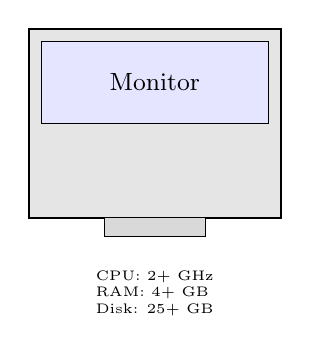
\begin{tikzpicture}[scale=0.8]
    % Computer
    \draw[fill=gray!20, thick] (0,0) rectangle (4,3);
    \draw[fill=blue!10] (0.2,1.5) rectangle (3.8,2.8);
    \node at (2,2.15) {\small Monitor};
    
    % Base
    \draw[fill=gray!30] (1.2,0) rectangle (2.8,-0.3);
    
    % Specs
    \node[align=left, font=\tiny] at (2,-1.2) {
        CPU: 2+ GHz\\
        RAM: 4+ GB\\
        Disk: 25+ GB
    };
\end{tikzpicture}

\vspace{0.3cm}

\textbf{Verifica compatibilità:}
\begin{itemize}
    \item Ubuntu Certified Hardware
    \item Linux Hardware Database
\end{itemize}
\end{columns}
\end{frame}

% Slide 4: Scelta della Distribuzione
\begin{frame}{Scegliere la Distribuzione Giusta}
\begin{table}
\small
\begin{tabular}{p{2.5cm}p{3.5cm}p{3.5cm}p{2cm}}
\toprule
\textbf{Distro} & \textbf{Vantaggi} & \textbf{Ideale per} & \textbf{Difficoltà} \\
\midrule
\textcolor{ubuntuorange}{\textbf{Ubuntu}} & 
- Facile da usare\newline
- Ampia documentazione\newline
- Supporto hardware & 
Principianti, Desktop, Sviluppatori & 
Bassa \\
\midrule
\textcolor{debianred}{\textbf{Debian}} & 
- Stabilissima\newline
- Repository enormi\newline
- Base per molte distro & 
Server, Utenti esperti & 
Media \\
\midrule
\textcolor{fedorablue}{\textbf{Fedora}} & 
- Tecnologie recenti\newline
- Base per RHEL\newline
- Innovativa & 
Sviluppatori, Workstation & 
Media \\
\bottomrule
\end{tabular}
\end{table}

\vspace{0.3cm}

\textbf{Fattori di scelta:}
\begin{itemize}
    \item Esperienza utente
    \item Scopo (desktop, server, sviluppo)
    \item Ciclo di aggiornamento preferito
    \item Supporto commerciale necessario
\end{itemize}
\end{frame}

% Slide 5: Download delle ISO
\begin{frame}{Download delle Immagini ISO}
\begin{columns}
\column{0.6\textwidth}
\textbf{Fonti ufficiali:}

\begin{enumerate}
    \item \textbf{Ubuntu}
    \begin{itemize}
        \item \texttt{ubuntu.com/download}
        \item Desktop, Server, varianti
        \item Scegliere LTS per stabilità
    \end{itemize}
    
    \item \textbf{Debian}
    \begin{itemize}
        \item \texttt{debian.org/download}
        \item Netinst (piccola), DVD (completa)
        \item Versioni: Stable, Testing
    \end{itemize}
    
    \item \textbf{Fedora}
    \begin{itemize}
        \item \texttt{getfedora.org}
        \item Workstation, Server, IoT
        \item Spin per diversi DE
    \end{itemize}
\end{enumerate}

\column{0.4\textwidth}
\textbf{Verifica integrità:}

\begin{lstlisting}[language=bash, basicstyle=\ttfamily\tiny, escapeinside={(*}{*)}]
(*\#*) Checksum SHA256
sha256sum ubuntu.iso

(*\#*) Confronta con file .sha256
cat ubuntu.iso.sha256
\end{lstlisting}

\vspace{0.3cm}

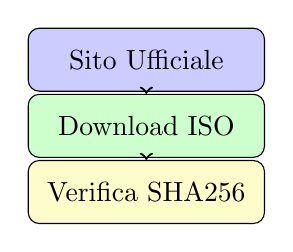
\begin{tikzpicture}[scale=0.7]
    \node[draw, rounded corners, fill=blue!20, minimum width=3cm, minimum height=0.8cm] (web) at (0,2) {Sito Ufficiale};
    \node[draw, rounded corners, fill=green!20, minimum width=3cm, minimum height=0.8cm] (iso) at (0,0.8) {Download ISO};
    \node[draw, rounded corners, fill=yellow!20, minimum width=3cm, minimum height=0.8cm] (check) at (0,-0.4) {Verifica SHA256};
    
    \draw[->, thick] (web) -- (iso);
    \draw[->, thick] (iso) -- (check);
\end{tikzpicture}
\end{columns}

\vspace{0.2cm}
\textbf{Attenzione:} Scaricare sempre da fonti ufficiali per sicurezza!
\end{frame}

% Slide 6: Creazione Media di Installazione
\begin{frame}{Creazione USB Avviabile}
\begin{columns}
\column{0.5\textwidth}
\textbf{Strumenti consigliati:}

\textbf{Windows:}
\begin{itemize}
    \item Rufus (consigliato)
    \item balenaEtcher
    \item UNetbootin
\end{itemize}

\textbf{Linux:}
\begin{itemize}
    \item dd (comando)
    \item GNOME Disks
    \item balenaEtcher
\end{itemize}

\textbf{macOS:}
\begin{itemize}
    \item balenaEtcher
    \item dd (comando)
\end{itemize}

\column{0.5\textwidth}
\textbf{Con dd (Linux/macOS):}

\begin{lstlisting}[language=bash, basicstyle=\ttfamily\tiny, escapeinside={(*}{*)}]
(*\#*) Identificare USB
lsblk

(*\#*) Smontare (se montato)
sudo umount /dev/sdX*

(*\#*) Scrivere immagine
sudo dd if=ubuntu.iso \
  of=/dev/sdX \
  bs=4M \
  status=progress

(*\#*) Sincronizzare
sync
\end{lstlisting}

\vspace{0.2cm}

\begin{block}{Attenzione}
\textbf{IMPORTANTE:} Verificare attentamente il dispositivo di destinazione (\texttt{/dev/sdX})! 
Il comando dd sovrascrive completamente il dispositivo.
\end{block}
\end{columns}
\end{frame}

% Slide 7: Modalità di Boot
\begin{frame}{Configurazione BIOS/UEFI}
\begin{columns}
\column{0.5\textwidth}
\textbf{Boot da USB:}

\begin{enumerate}
    \item Riavviare il computer
    \item Premere tasto di boot:
    \begin{itemize}
        \item F12 (Dell, Lenovo)
        \item F9 (HP)
        \item Esc, F2, Del (altri)
    \end{itemize}
    \item Selezionare USB
    \item Avviare
\end{enumerate}

\vspace{0.3cm}

\textbf{UEFI vs Legacy BIOS:}
\begin{itemize}
    \item \textbf{UEFI:} Moderno, Secure Boot, GPT
    \item \textbf{Legacy:} Vecchio, BIOS, MBR
    \item Preferire UEFI su hardware recente
\end{itemize}

\column{0.5\textwidth}
\textbf{Secure Boot:}

\begin{itemize}
    \item Verifica firma digitale
    \item Ubuntu/Fedora: supporto nativo
    \item Debian: richiede shim-signed
    \item Può essere disabilitato se problematico
\end{itemize}

\vspace{0.3cm}

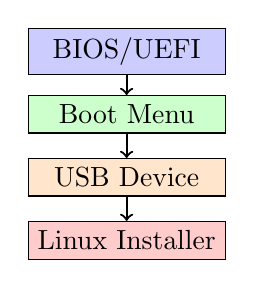
\begin{tikzpicture}[scale=0.8]
    \node[draw, rectangle, fill=blue!20, minimum width=2.5cm] (bios) at (0,2) {BIOS/UEFI};
    \node[draw, rectangle, fill=green!20, minimum width=2.5cm] (boot) at (0,1) {Boot Menu};
    \node[draw, rectangle, fill=orange!20, minimum width=2.5cm] (usb) at (0,0) {USB Device};
    \node[draw, rectangle, fill=red!20, minimum width=2.5cm] (linux) at (0,-1) {Linux Installer};
    
    \draw[->, thick] (bios) -- (boot);
    \draw[->, thick] (boot) -- (usb);
    \draw[->, thick] (usb) -- (linux);
\end{tikzpicture}
\end{columns}
\end{frame}

\section{Installazione Ubuntu}

% Slide 8: Avvio Installer Ubuntu
\begin{frame}{Ubuntu: Avvio dell'Installazione}
\begin{columns}
\column{0.5\textwidth}
\textbf{Schermata iniziale:}

\begin{enumerate}
    \item \textbf{Try Ubuntu} - Live session
    \begin{itemize}
        \item Testare senza installare
        \item Verificare hardware
        \item Navigare in internet
    \end{itemize}
    
    \item \textbf{Install Ubuntu} - Installazione diretta
    \begin{itemize}
        \item Processo guidato
        \item Circa 15-30 minuti
    \end{itemize}
\end{enumerate}

\vspace{0.3cm}

\textbf{Scelte iniziali:}
\begin{itemize}
    \item Lingua dell'interfaccia
    \item Layout tastiera
    \item Connessione WiFi (opzionale)
\end{itemize}

\column{0.5\textwidth}
\textbf{Opzioni di installazione:}

\begin{itemize}
    \item \textbf{Installazione normale}
    \begin{itemize}
        \item Browser, suite office, media player
        \item Giochi, utility
    \end{itemize}
    
    \item \textbf{Installazione minima}
    \begin{itemize}
        \item Solo essenziali
        \item Browser e utility base
        \item Sistema più leggero
    \end{itemize}
\end{itemize}

\vspace{0.3cm}

\textbf{Aggiornamenti durante installazione:}
\begin{itemize}
    \item[$\square$] Scaricare aggiornamenti
    \item[$\square$] Installare software di terze parti
    \begin{itemize}
        \item Driver proprietari
        \item Codec multimediali
    \end{itemize}
\end{itemize}
\end{columns}
\end{frame}

% Slide 9: Partizionamento Ubuntu
\begin{frame}{Ubuntu: Partizionamento del Disco}
\begin{columns}
\column{0.5\textwidth}
\textbf{Opzioni disponibili:}

\begin{enumerate}
    \item \textbf{Cancella disco e installa Ubuntu}
    \begin{itemize}
        \item Più semplice
        \item Partizionamento automatico
        \item Cancella tutto
    \end{itemize}
    
    \item \textbf{Installa insieme a Windows}
    \begin{itemize}
        \item Dual boot
        \item Ridimensiona partizione esistente
        \item Mantiene Windows
    \end{itemize}
    
    \item \textbf{Altro (Manuale)}
    \begin{itemize}
        \item Controllo completo
        \item Per utenti esperti
    \end{itemize}
\end{enumerate}

\column{0.5\textwidth}
\textbf{Schema partizioni manuale:}

\begin{table}
\tiny
\begin{tabular}{llll}
\toprule
\textbf{Mount} & \textbf{Tipo} & \textbf{Dim.} & \textbf{Flag} \\
\midrule
/boot/efi & FAT32 & 512 MB & boot, esp \\
/ & ext4 & 50+ GB & - \\
/home & ext4 & resto & - \\
swap & swap & 4-8 GB & - \\
\bottomrule
\end{tabular}
\end{table}

\vspace{0.2cm}

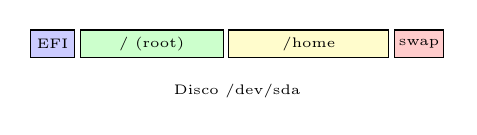
\begin{tikzpicture}[scale=0.7]
    \draw[fill=blue!20] (0,0) rectangle (0.8,0.5);
    \node[font=\tiny] at (0.4,0.25) {EFI};
    
    \draw[fill=green!20] (0.9,0) rectangle (3.5,0.5);
    \node[font=\tiny] at (2.2,0.25) {/ (root)};
    
    \draw[fill=yellow!20] (3.6,0) rectangle (6.5,0.5);
    \node[font=\tiny] at (5.05,0.25) {/home};
    
    \draw[fill=red!20] (6.6,0) rectangle (7.5,0.5);
    \node[font=\tiny] at (7.05,0.25) {swap};
    
    \node[font=\tiny, below] at (3.75,-0.3) {Disco /dev/sda};
\end{tikzpicture}
\end{columns}

\vspace{0.2cm}
\textbf{LVM e cifratura:}
\begin{itemize}
    \item Opzione per LVM (Logical Volume Manager)
    \item Cifratura disco per sicurezza
\end{itemize}
\end{frame}

% Slide 10: Configurazione Utente Ubuntu
\begin{frame}{Ubuntu: Configurazione Utente e Completamento}
\begin{columns}
\column{0.5\textwidth}
\textbf{Creazione account:}

\begin{itemize}
    \item Nome completo
    \item Nome computer
    \item Username
    \item Password (forte!)
    \item Conferma password
\end{itemize}

\vspace{0.3cm}

\textbf{Opzioni di login:}
\begin{itemize}
    \item[$\circ$] Richiedere password al login
    \item[$\circ$] Login automatico
\end{itemize}

\vspace{0.3cm}

\textbf{Installazione:}
\begin{itemize}
    \item Copia file (15-20 min)
    \item Configurazione sistema
    \item Installazione bootloader (GRUB)
\end{itemize}

\column{0.5\textwidth}
\textbf{Post-installazione:}

\begin{enumerate}
    \item Riavvio sistema
    \item Rimozione USB
    \item Primo login
    \item Configurazione online accounts (opzionale)
    \item Configurazione Livepatch (opzionale)
    \item Tour iniziale
\end{enumerate}

\vspace{0.3cm}

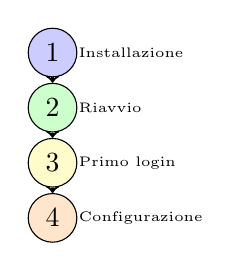
\begin{tikzpicture}[scale=0.7]
    \node[draw, circle, fill=blue!20] (1) at (0,2) {1};
    \node[right, font=\tiny] at (0.3,2) {Installazione};
    
    \node[draw, circle, fill=green!20] (2) at (0,1) {2};
    \node[right, font=\tiny] at (0.3,1) {Riavvio};
    
    \node[draw, circle, fill=yellow!20] (3) at (0,0) {3};
    \node[right, font=\tiny] at (0.3,0) {Primo login};
    
    \node[draw, circle, fill=orange!20] (4) at (0,-1) {4};
    \node[right, font=\tiny] at (0.3,-1) {Configurazione};
    
    \draw[->, thick] (1) -- (2);
    \draw[->, thick] (2) -- (3);
    \draw[->, thick] (3) -- (4);
\end{tikzpicture}
\end{columns}
\end{frame}

\section{Installazione Debian}

% Slide 11: Debian Installer - Introduzione
\begin{frame}{Debian: Processo di Installazione}
\begin{columns}
\column{0.5\textwidth}
\textbf{Caratteristiche installer:}

\begin{itemize}
    \item Interfaccia testuale/grafica
    \item Più opzioni di configurazione
    \item Processo più dettagliato
    \item Maggiore controllo
\end{itemize}

\vspace{0.3cm}

\textbf{Modalità disponibili:}
\begin{enumerate}
    \item Graphical install
    \item Install (testuale)
    \item Advanced options
    \begin{itemize}
        \item Expert install
        \item Rescue mode
        \item Automated install
    \end{itemize}
\end{enumerate}

\column{0.5\textwidth}
\textbf{Fasi principali:}

\begin{enumerate}
    \item Selezione lingua e località
    \item Configurazione tastiera
    \item Configurazione rete
    \item Configurazione hostname
    \item Configurazione dominio
    \item Impostazione password root
    \item Creazione utente
    \item Partizionamento
    \item Selezione mirror
    \item Selezione software
    \item Installazione GRUB
\end{enumerate}
\end{columns}

\vspace{0.2cm}
\textbf{Tempo richiesto:} 20-40 minuti (dipende da connessione e scelte)
\end{frame}

% Slide 12: Debian - Configurazione Rete e Utenti
\begin{frame}{Debian: Configurazione Rete e Utenti}
\begin{columns}
\column{0.5\textwidth}
\textbf{Configurazione rete:}

\begin{itemize}
    \item \textbf{Hostname}
    \begin{itemize}
        \item Nome del computer
        \item Es: \texttt{debian-pc}
    \end{itemize}
    
    \item \textbf{Dominio}
    \begin{itemize}
        \item Opzionale per desktop
        \item Necessario per server
        \item Può essere lasciato vuoto
    \end{itemize}
    
    \item \textbf{Mirror Debian}
    \begin{itemize}
        \item Selezione paese
        \item Scelta mirror specifico
        \item Proxy HTTP (se necessario)
    \end{itemize}
\end{itemize}

\column{0.5\textwidth}
\textbf{Account utenti:}

\begin{enumerate}
    \item \textbf{Password root}
    \begin{itemize}
        \item Account amministratore
        \item Password forte
        \item Può essere lasciata vuota (usa sudo)
    \end{itemize}
    
    \item \textbf{Utente normale}
    \begin{itemize}
        \item Nome completo
        \item Username
        \item Password
    \end{itemize}
\end{enumerate}

\vspace{0.3cm}

\begin{block}{Suggerimento}
Se la password root è vuota, l'utente creato avrà privilegi sudo automaticamente.
\end{block}
\end{columns}
\end{frame}

% Slide 13: Debian - Partizionamento
\begin{frame}{Debian: Opzioni di Partizionamento}
\begin{columns}
\column{0.5\textwidth}
\textbf{Metodi guidati:}

\begin{enumerate}
    \item \textbf{Tutto in una partizione}
    \begin{itemize}
        \item Più semplice
        \item Una sola partizione per tutto
    \end{itemize}
    
    \item \textbf{Partizione /home separata}
    \begin{itemize}
        \item Dati utente separati
        \item Facilita reinstallazioni
    \end{itemize}
    
    \item \textbf{Partizioni separate /home, /var, /tmp}
    \begin{itemize}
        \item Massima separazione
        \item Migliore per server
    \end{itemize}
\end{enumerate}

\vspace{0.3cm}

\textbf{Opzioni avanzate:}
\begin{itemize}
    \item LVM (Logical Volume Manager)
    \item LVM cifrato
    \item Partizionamento manuale
\end{itemize}

\column{0.5\textwidth}
\textbf{Filesystem supportati:}

\begin{itemize}
    \item \textbf{ext4} - Standard Linux (consigliato)
    \item \textbf{ext3} - Compatibilità legacy
    \item \textbf{XFS} - Performance su file grandi
    \item \textbf{Btrfs} - Moderno, snapshot
    \item \textbf{JFS} - Journaling IBM
    \item \textbf{FAT32/VFAT} - Boot EFI, compatibilità
\end{itemize}

\vspace{0.3cm}

\textbf{Partizionamento manuale:}
\begin{itemize}
    \item Controllo completo
    \item Creazione/modifica partizioni
    \item Punti di mount personalizzati
    \item Flag e opzioni avanzate
\end{itemize}
\end{columns}
\end{frame}

% Slide 14: Debian - Selezione Software
\begin{frame}{Debian: Selezione Software e Tasksel}
\begin{columns}
\column{0.5\textwidth}
\textbf{Desktop Environment:}

\begin{itemize}
    \item[$\square$] Debian desktop environment
    \item[$\square$] GNOME
    \item[$\square$] Xfce
    \item[$\square$] KDE Plasma
    \item[$\square$] Cinnamon
    \item[$\square$] MATE
    \item[$\square$] LXDE
    \item[$\square$] LXQt
\end{itemize}

\vspace{0.3cm}

\textbf{Altri task:}
\begin{itemize}
    \item[$\square$] Web server
    \item[$\square$] SSH server
    \item[$\square$] Standard system utilities
\end{itemize}

\column{0.5\textwidth}
\textbf{Considerazioni:}

\begin{itemize}
    \item Selezionare solo uno DE principale
    \item "Debian desktop" installa GNOME
    \item Sistema minimo: deselezionare tutti i DE
    \item SSH utile per server
    \item Standard utilities quasi sempre necessario
\end{itemize}

\vspace{0.3cm}

\textbf{Post-installazione con tasksel:}

\begin{lstlisting}[language=bash, basicstyle=\ttfamily\tiny, escapeinside={(*}{*)}]
(*\#*) Eseguire dopo installazione
sudo tasksel

(*\#*) Da terminale
sudo tasksel install kde-desktop
sudo tasksel remove gnome-desktop
\end{lstlisting}
\end{columns}

\vspace{0.2cm}
\textbf{Nota:} Scelte possono essere modificate dopo installazione
\end{frame}

\section{Installazione Fedora}

% Slide 15: Fedora Anaconda Installer
\begin{frame}{Fedora: Anaconda Installer}
\begin{columns}
\column{0.5\textwidth}
\textbf{Caratteristiche Anaconda:}

\begin{itemize}
    \item Interfaccia grafica moderna
    \item Hub-and-spoke model
    \item Configurazione parallela
    \item Anteprima in tempo reale
\end{itemize}

\vspace{0.3cm}

\textbf{Schermata principale (Hub):}

Elementi da configurare:
\begin{enumerate}
    \item Tastiera
    \item Lingua e supporto
    \item Data e ora
    \item Destinazione installazione
    \item Rete e hostname
    \item Software selection (opzionale)
\end{enumerate}

\column{0.5\textwidth}
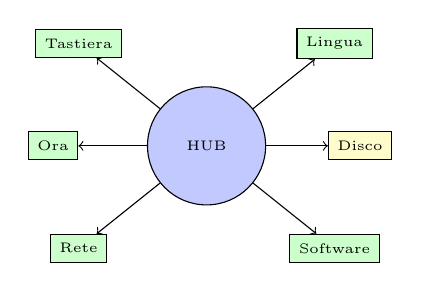
\begin{tikzpicture}[scale=0.65]
    % Hub centrale
    \node[draw, circle, fill=fedorablue!30, minimum size=1.5cm] (hub) at (0,0) {\tiny HUB};
    
    % Spokes
    \node[draw, rectangle, fill=green!20, font=\tiny] (kbd) at (-2.5,2) {Tastiera};
    \node[draw, rectangle, fill=green!20, font=\tiny] (lang) at (2.5,2) {Lingua};
    \node[draw, rectangle, fill=green!20, font=\tiny] (time) at (-3,0) {Ora};
    \node[draw, rectangle, fill=yellow!20, font=\tiny] (disk) at (3,0) {Disco};
    \node[draw, rectangle, fill=green!20, font=\tiny] (net) at (-2.5,-2) {Rete};
    \node[draw, rectangle, fill=green!20, font=\tiny] (soft) at (2.5,-2) {Software};
    
    % Connessioni
    \draw[->] (hub) -- (kbd);
    \draw[->] (hub) -- (lang);
    \draw[->] (hub) -- (time);
    \draw[->] (hub) -- (disk);
    \draw[->] (hub) -- (net);
    \draw[->] (hub) -- (soft);
\end{tikzpicture}

\vspace{0.2cm}

\textbf{Icone di stato:}
\begin{itemize}
    \item \textcolor{green}{[OK]} Configurato
    \item \textcolor{orange}{[!]} Attenzione richiesta
    \item \textcolor{red}{[X]} Configurazione obbligatoria
\end{itemize}
\end{columns}

\vspace{0.2cm}
\textbf{Nota:} Non è necessario seguire un ordine specifico
\end{frame}

% Slide 16: Fedora - Partizionamento
\begin{frame}{Fedora: Configurazione Storage}
\begin{columns}
\column{0.5\textwidth}
\textbf{Opzioni di storage:}

\begin{enumerate}
    \item \textbf{Automatico}
    \begin{itemize}
        \item Configurazione standard
        \item Usa LVM di default
        \item Btrfs come filesystem
    \end{itemize}
    
    \item \textbf{Personalizzato}
    \begin{itemize}
        \item Controllo completo
        \item Schema partizioni manuale
        \item Scelta filesystem
    \end{itemize}
\end{enumerate}

\vspace{0.3cm}

\textbf{Opzioni di cifratura:}
\begin{itemize}
    \item[$\square$] Cifra i miei dati
    \item Password di cifratura
    \item LUKS (Linux Unified Key Setup)
\end{itemize}

\column{0.5\textwidth}
\textbf{Schema automatico con LVM:}

\begin{table}
\tiny
\begin{tabular}{lll}
\toprule
\textbf{Volume} & \textbf{FS} & \textbf{Dimensione} \\
\midrule
/boot/efi & vfat & 600 MB \\
/boot & ext4 & 1 GB \\
/ & btrfs & 15+ GB \\
/home & btrfs & resto \\
swap & swap & 4-8 GB \\
\bottomrule
\end{tabular}
\end{table}

\vspace{0.2cm}

\textbf{Filesystem Btrfs:}
\begin{itemize}
    \item Default in Fedora 33+
    \item Snapshot e rollback
    \item Compressione trasparente
    \item Subvolume per /home
\end{itemize}
\end{columns}

\vspace{0.2cm}
\textbf{Recupero spazio:} Opzioni per ridimensionare/eliminare partizioni esistenti
\end{frame}

% Slide 17: Fedora - Completamento
\begin{frame}{Fedora: Creazione Utente e Completamento}
\begin{columns}
\column{0.5\textwidth}
\textbf{Durante installazione:}

\begin{itemize}
    \item Click su "Begin Installation"
    \item Installazione inizia
    \item Configurazione utente in parallelo:
    \begin{enumerate}
        \item Root Password (opzionale)
        \item User Creation (obbligatorio)
    \end{enumerate}
\end{itemize}

\vspace{0.3cm}

\textbf{Creazione utente:}
\begin{itemize}
    \item Nome completo
    \item Username
    \item Password
    \item[$\square$] Rendi amministratore (sudo)
    \item[$\square$] Richiedi password per login
\end{itemize}

\column{0.5\textwidth}
\textbf{Primo avvio:}

\begin{enumerate}
    \item GNOME Initial Setup
    \item Connessione online accounts
    \begin{itemize}
        \item Google
        \item Microsoft
        \item Nextcloud
        \item Altri
    \end{itemize}
    \item Configurazione privacy
    \item Enable Third Party Repositories
    \item Completamento configurazione
\end{enumerate}

\vspace{0.3cm}

\begin{block}{Third Party Repos}
Include driver NVIDIA, codec multimediali, Chrome, Steam, ecc.
\end{block}
\end{columns}
\end{frame}

\section{Gestione Pacchetti}

% Slide 18: Introduzione Package Management
\begin{frame}{Sistemi di Gestione Pacchetti}
\begin{columns}
\column{0.5\textwidth}
\textbf{Concetti fondamentali:}

\begin{itemize}
    \item \textbf{Pacchetto:} Software impacchettato
    \item \textbf{Repository:} Server con pacchetti
    \item \textbf{Dipendenze:} Librerie necessarie
    \item \textbf{Package Manager:} Tool di gestione
\end{itemize}

\vspace{0.3cm}

\textbf{Livelli di gestione:}

\begin{enumerate}
    \item \textbf{Low-level} (dpkg, rpm)
    \begin{itemize}
        \item Installazione pacchetti locali
        \item Non gestisce dipendenze
        \item Non scarica da repository
    \end{itemize}
    
    \item \textbf{High-level} (apt, dnf)
    \begin{itemize}
        \item Risolve dipendenze
        \item Scarica da repository
        \item Gestione completa
    \end{itemize}
\end{enumerate}

\column{0.5\textwidth}
\textbf{Sistemi principali:}

\begin{table}
\small
\begin{tabular}{lll}
\toprule
\textbf{Distro} & \textbf{Low} & \textbf{High} \\
\midrule
Debian & dpkg & apt \\
Ubuntu & dpkg & apt \\
Fedora & rpm & dnf \\
RHEL & rpm & yum/dnf \\
Arch & - & pacman \\
\bottomrule
\end{tabular}
\end{table}

\vspace{0.3cm}

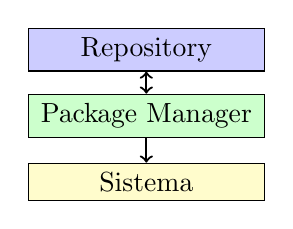
\begin{tikzpicture}[scale=0.7]
    \node[draw, rectangle, fill=blue!20, minimum width=3cm] (repo) at (0,2) {Repository};
    \node[draw, rectangle, fill=green!20, minimum width=3cm] (pm) at (0,0.8) {Package Manager};
    \node[draw, rectangle, fill=yellow!20, minimum width=3cm] (sys) at (0,-0.4) {Sistema};
    
    \draw[<->, thick] (repo) -- (pm);
    \draw[->, thick] (pm) -- (sys);
\end{tikzpicture}
\end{columns}
\end{frame}

% Slide 19: APT - Debian/Ubuntu
\begin{frame}[fragile]{APT: Advanced Package Tool}
\begin{columns}
\column{0.5\textwidth}
\textbf{Comandi principali:}

\begin{lstlisting}[language=bash, basicstyle=\ttfamily\tiny, escapeinside={(*}{*)}]
(*\#*) Aggiornare lista pacchetti
sudo apt update

(*\#*) Aggiornare sistema
sudo apt upgrade

(*\#*) Aggiornamento completo
sudo apt full-upgrade

(*\#*) Installare pacchetto
sudo apt install nome-pacchetto

(*\#*) Rimuovere pacchetto
sudo apt remove nome-pacchetto

(*\#*) Rimuovere + configurazioni
sudo apt purge nome-pacchetto

(*\#*) Rimuovere dipendenze inutili
sudo apt autoremove
\end{lstlisting}

\column{0.5\textwidth}
\textbf{Ricerca e informazioni:}

\begin{lstlisting}[language=bash, basicstyle=\ttfamily\tiny, escapeinside={(*}{*)}]
(*\#*) Cercare pacchetto
apt search termine

(*\#*) Info su pacchetto
apt show nome-pacchetto

(*\#*) Elencare file in pacchetto
dpkg -L nome-pacchetto

(*\#*) Trovare pacchetto da file
dpkg -S /path/to/file

(*\#*) Lista pacchetti installati
apt list --installed

(*\#*) Pacchetti aggiornabili
apt list --upgradable
\end{lstlisting}

\vspace{0.3cm}

\textbf{File di configurazione:}
\begin{itemize}
    \item \texttt{/etc/apt/sources.list}
    \item \texttt{/etc/apt/sources.list.d/}
\end{itemize}
\end{columns}
\end{frame}

% Slide 20: Repository Debian/Ubuntu
\begin{frame}[fragile]{Gestione Repository in Debian/Ubuntu}
\begin{columns}
\column{0.5\textwidth}
\textbf{Struttura sources.list:}

\begin{lstlisting}[basicstyle=\ttfamily\tiny]
(*\#*) Ubuntu main repository
deb http://archive.ubuntu.com/ubuntu/ jammy main restricted

deb http://archive.ubuntu.com/ubuntu/ jammy-updates main restricted

deb http://archive.ubuntu.com/ubuntu/ jammy universe

deb http://archive.ubuntu.com/ubuntu/ jammy-security main restricted
\end{lstlisting}

\vspace{0.3cm}

\textbf{Componenti Ubuntu:}
\begin{itemize}
    \item \textbf{main} - Supportato ufficialmente
    \item \textbf{restricted} - Driver proprietari
    \item \textbf{universe} - Community
    \item \textbf{multiverse} - Software non-free
\end{itemize}

\column{0.5\textwidth}
\textbf{Aggiungere repository:}

\begin{lstlisting}[language=bash, basicstyle=\ttfamily\tiny, escapeinside={(*}{*)}]
(*\#*) PPA (Personal Package Archive)
sudo add-apt-repository ppa:user/ppa-name
sudo apt update

(*\#*) Repository manuale
echo "deb [arch=amd64] http://..." | \
  sudo tee /etc/apt/sources.list.d/repo.list

(*\#*) Aggiungere chiave GPG
wget -qO- https://url/key.gpg | \
  sudo gpg --dearmor -o \
  /etc/apt/trusted.gpg.d/repo.gpg
\end{lstlisting}

\vspace{0.3cm}

\textbf{Rimuovere repository:}
\begin{lstlisting}[language=bash, basicstyle=\ttfamily\tiny, escapeinside={(*}{*)}]
sudo add-apt-repository --remove ppa:user/ppa-name
(*\#*) oppure modificare/eliminare file in sources.list.d/
\end{lstlisting}
\end{columns}
\end{frame}

% Slide 21: DNF - Fedora
\begin{frame}[fragile]{DNF: Dandified Yum}
\begin{columns}
\column{0.5\textwidth}
\textbf{Comandi base:}

\begin{lstlisting}[language=bash, basicstyle=\ttfamily\tiny, escapeinside={(*}{*)}]
(*\#*) Aggiornare cache metadata
sudo dnf check-update

(*\#*) Aggiornare sistema
sudo dnf upgrade

(*\#*) Installare pacchetto
sudo dnf install nome-pacchetto

(*\#*) Rimuovere pacchetto
sudo dnf remove nome-pacchetto

(*\#*) Rimuovere dipendenze inutili
sudo dnf autoremove

(*\#*) Cercare pacchetto
dnf search termine

(*\#*) Info pacchetto
dnf info nome-pacchetto
\end{lstlisting}

\column{0.5\textwidth}
\textbf{Comandi avanzati:}

\begin{lstlisting}[language=bash, basicstyle=\ttfamily\tiny, escapeinside={(*}{*)}]
(*\#*) Gruppi di pacchetti
dnf group list
dnf group install "Development Tools"

(*\#*) Cronologia transazioni
dnf history

(*\#*) Rollback transazione
sudo dnf history undo <ID>

(*\#*) Lista file in pacchetto
dnf repoquery -l nome-pacchetto

(*\#*) Pacchetto che fornisce file
dnf provides /path/to/file

(*\#*) Pulizia cache
sudo dnf clean all
\end{lstlisting}

\vspace{0.3cm}

\textbf{Differenze da yum:}
\begin{itemize}
    \item Più veloce
    \item Migliore risoluzione dipendenze
    \item API Python moderna
\end{itemize}
\end{columns}
\end{frame}

% Slide 22: Repository Fedora
\begin{frame}[fragile]{Repository in Fedora}
\begin{columns}
\column{0.5\textwidth}
\textbf{Repository ufficiali:}

\begin{itemize}
    \item \textbf{fedora} - Software release
    \item \textbf{updates} - Aggiornamenti
    \item \textbf{updates-testing} - Test
\end{itemize}

\vspace{0.3cm}

\textbf{Repository terze parti:}

\begin{enumerate}
    \item \textbf{RPM Fusion}
    \begin{lstlisting}[language=bash, basicstyle=\ttfamily\tiny, escapeinside={(*}{*)}]
(*\#*) Free
sudo dnf install \
  https://download1.rpmfusion.org/free/fedora/rpmfusion-free-release-$(rpm -E %fedora).noarch.rpm

(*\#*) Nonfree
sudo dnf install \
  https://download1.rpmfusion.org/nonfree/fedora/rpmfusion-nonfree-release-$(rpm -E %fedora).noarch.rpm
    \end{lstlisting}
    
    \item \textbf{COPR} (Community repos)
    \begin{lstlisting}[language=bash, basicstyle=\ttfamily\tiny, escapeinside={(*}{*)}]
sudo dnf copr enable user/project
    \end{lstlisting}
\end{enumerate}

\column{0.5\textwidth}
\textbf{Gestione repository:}

\begin{lstlisting}[language=bash, basicstyle=\ttfamily\tiny, escapeinside={(*}{*)}]
(*\#*) Elencare repository
dnf repolist

(*\#*) Abilitare repository
sudo dnf config-manager --set-enabled repo-id

(*\#*) Disabilitare repository
sudo dnf config-manager --set-disabled repo-id

(*\#*) Aggiungere repository
sudo dnf config-manager --add-repo http://...
\end{lstlisting}

\vspace{0.3cm}

\textbf{File configurazione:}
\begin{itemize}
    \item \texttt{/etc/yum.repos.d/}
    \item File \texttt{.repo}
\end{itemize}

\begin{lstlisting}[basicstyle=\ttfamily\tiny]
[repository-name]
name=Repository Name
baseurl=http://...
enabled=1
gpgcheck=1
gpgkey=file:///etc/pki/...
\end{lstlisting}
\end{columns}
\end{frame}

% Slide 23: Flatpak
\begin{frame}[fragile]{Flatpak: Applicazioni Universali}
\begin{columns}
\column{0.5\textwidth}
\textbf{Cos'è Flatpak?}

\begin{itemize}
    \item Sistema distribuzione app universale
    \item Sandbox per sicurezza
    \item Runtime condivisi
    \item Indipendente da distribuzione
    \item Aggiornamenti gestiti separatamente
\end{itemize}

\vspace{0.3cm}

\textbf{Installazione:}

\begin{lstlisting}[language=bash, basicstyle=\ttfamily\tiny, escapeinside={(*}{*)}]
(*\#*) Debian/Ubuntu
sudo apt install flatpak

(*\#*) Fedora (già incluso)
sudo dnf install flatpak

(*\#*) Aggiungere Flathub
flatpak remote-add --if-not-exists flathub https://flathub.org/repo/flathub.flatpakrepo
\end{lstlisting}

\column{0.5\textwidth}
\textbf{Comandi comuni:}

\begin{lstlisting}[language=bash, basicstyle=\ttfamily\tiny, escapeinside={(*}{*)}]
(*\#*) Cercare app
flatpak search nome

(*\#*) Installare app
flatpak install flathub com.app.Name

(*\#*) Eseguire app
flatpak run com.app.Name

(*\#*) Lista app installate
flatpak list

(*\#*) Aggiornare tutte le app
flatpak update

(*\#*) Rimuovere app
flatpak uninstall com.app.Name

(*\#*) Rimuovere runtime inutilizzati
flatpak uninstall --unused
\end{lstlisting}

\vspace{0.3cm}

\textbf{Vantaggi:}
\begin{itemize}
    \item Software sempre aggiornato
    \item Isolamento sicurezza
    \item Funziona su tutte le distro
\end{itemize}
\end{columns}
\end{frame}

% Slide 24: Snap
\begin{frame}[fragile]{Snap: Sistema Pacchetti Canonical}
\begin{columns}
\column{0.5\textwidth}
\textbf{Caratteristiche Snap:}

\begin{itemize}
    \item Sviluppato da Canonical
    \item Pacchetti autocontenuti
    \item Aggiornamenti automatici
    \item Rollback versioni precedenti
    \item Canali: stable, candidate, beta, edge
\end{itemize}

\vspace{0.3cm}

\textbf{Installazione snapd:}

\begin{lstlisting}[language=bash, basicstyle=\ttfamily\tiny, escapeinside={(*}{*)}]
(*\#*) Ubuntu (preinstallato)

(*\#*) Debian
sudo apt install snapd
sudo systemctl enable --now snapd

(*\#*) Fedora
sudo dnf install snapd
sudo ln -s /var/lib/snapd/snap /snap
\end{lstlisting}

\column{0.5\textwidth}
\textbf{Comandi snap:}

\begin{lstlisting}[language=bash, basicstyle=\ttfamily\tiny, escapeinside={(*}{*)}]
(*\#*) Cercare snap
snap find termine

(*\#*) Installare snap
sudo snap install nome-snap

(*\#*) Installare da canale specifico
sudo snap install nome --edge

(*\#*) Lista snap installati
snap list

(*\#*) Info snap
snap info nome-snap

(*\#*) Aggiornare snap
sudo snap refresh nome-snap

(*\#*) Rimuovere snap
sudo snap remove nome-snap

(*\#*) Disabilitare aggiornamenti auto
sudo snap refresh --hold
\end{lstlisting}

\vspace{0.2cm}

\textbf{Confinamento:}
\begin{itemize}
    \item strict - Isolamento completo
    \item classic - Accesso completo
    \item devmode - Sviluppo
\end{itemize}
\end{columns}
\end{frame}

% Slide 25: AppImage
\begin{frame}{AppImage: Applicazioni Portable}
\begin{columns}
\column{0.5\textwidth}
\textbf{Cos'è AppImage?}

\begin{itemize}
    \item Formato applicazioni portatili
    \item Un file eseguibile
    \item Nessuna installazione richiesta
    \item Tutte dipendenze incluse
    \item Esecuzione diretta
\end{itemize}

\vspace{0.3cm}

\textbf{Utilizzo:}

\begin{enumerate}
    \item Scaricare file .AppImage
    \item Rendere eseguibile:
    \begin{itemize}
        \item GUI: Click destro → Proprietà → Permessi
        \item CLI: \texttt{chmod +x file.AppImage}
    \end{itemize}
    \item Eseguire: \texttt{./file.AppImage}
\end{enumerate}

\column{0.5\textwidth}
\textbf{Vantaggi:}

\begin{itemize}
    \item Semplicità estrema
    \item Nessuna modifica al sistema
    \item Facilmente rimovibile
    \item Versioni multiple convivono
    \item Funziona su quasi tutte le distro
\end{itemize}

\vspace{0.3cm}

\textbf{Svantaggi:}

\begin{itemize}
    \item File più grandi
    \item Aggiornamenti manuali
    \item Nessuna integrazione sistema
    \item Possibile duplicazione librerie
\end{itemize}

\vspace{0.3cm}

\textbf{AppImageLauncher:}
\begin{itemize}
    \item Integrazione nel sistema
    \item Gestione AppImage
    \item Creazione shortcut
\end{itemize}
\end{columns}
\end{frame}

\section{Aggiornamenti di Sistema}

% Slide 26: Aggiornamenti Ubuntu
\begin{frame}[fragile]{Aggiornamenti in Ubuntu}
\begin{columns}
\column{0.5\textwidth}
\textbf{Tipi di aggiornamenti:}

\begin{enumerate}
    \item \textbf{Aggiornamenti di sicurezza}
    \begin{itemize}
        \item Priorità massima
        \item Automatici (opzionale)
    \end{itemize}
    
    \item \textbf{Aggiornamenti raccomandati}
    \begin{itemize}
        \item Bug fix
        \item Miglioramenti
    \end{itemize}
    
    \item \textbf{Aggiornamenti opzionali}
    \begin{itemize}
        \item Nuove funzionalità
        \item Software aggiuntivo
    \end{itemize}
\end{enumerate}

\vspace{0.3cm}

\textbf{Via GUI:}
\begin{itemize}
    \item Software Updater
    \item Notifiche automatiche
    \item Click per aggiornare
\end{itemize}

\column{0.5\textwidth}
\textbf{Via terminale:}

\begin{lstlisting}[language=bash, basicstyle=\ttfamily\tiny, escapeinside={(*}{*)}]
(*\#*) Aggiornamento completo
sudo apt update
sudo apt upgrade

(*\#*) Include rimozione pacchetti obsoleti
sudo apt full-upgrade

(*\#*) Pulizia
sudo apt autoremove
sudo apt autoclean
\end{lstlisting}

\vspace{0.3cm}

\textbf{Aggiornamenti automatici:}

\begin{lstlisting}[language=bash, basicstyle=\ttfamily\tiny, escapeinside={(*}{*)}]
(*\#*) Installare
sudo apt install unattended-upgrades

(*\#*) Configurare
sudo dpkg-reconfigure unattended-upgrades

(*\#*) File configurazione
/etc/apt/apt.conf.d/50unattended-upgrades
\end{lstlisting}

\vspace{0.2cm}

\textbf{Ubuntu Pro:}
\begin{itemize}
    \item Livepatch kernel (no riavvio)
    \item Supporto esteso
\end{itemize}
\end{columns}
\end{frame}

% Slide 27: Upgrade Ubuntu
\begin{frame}[fragile]{Upgrade di Versione in Ubuntu}
\begin{columns}
\column{0.5\textwidth}
\textbf{Tipi di upgrade:}

\begin{itemize}
    \item \textbf{LTS → LTS}
    \begin{itemize}
        \item Ogni 2 anni
        \item Più sicuro
        \item Raccomandato
    \end{itemize}
    
    \item \textbf{Normale → Normale}
    \begin{itemize}
        \item Ogni 6 mesi
        \item Più frequente
        \item Nuove funzionalità
    \end{itemize}
\end{itemize}

\vspace{0.3cm}

\textbf{Preparazione:}
\begin{enumerate}
    \item Backup dati importanti
    \item Aggiornare sistema corrente
    \item Rimuovere PPA problematici
    \item Verificare spazio disco
    \item Connessione stabile
\end{enumerate}

\column{0.5\textwidth}
\textbf{Procedura GUI:}
\begin{itemize}
    \item Software Updater
    \item Notifica nuova versione
    \item Click "Upgrade"
    \item Seguire procedura guidata
\end{itemize}

\vspace{0.3cm}

\textbf{Procedura CLI:}

\begin{lstlisting}[language=bash, basicstyle=\ttfamily\tiny, escapeinside={(*}{*)}]
(*\#*) Aggiornare sistema corrente
sudo apt update
sudo apt upgrade
sudo apt full-upgrade

(*\#*) Installare update-manager
sudo apt install update-manager-core

(*\#*) Avviare upgrade
sudo do-release-upgrade

(*\#*) Per versione sviluppo
sudo do-release-upgrade -d
\end{lstlisting}

\vspace{0.2cm}

\textbf{Tempo richiesto:}
\begin{itemize}
    \item Download: 15-30 min
    \item Installazione: 30-60 min
    \item Totale: 1-2 ore
\end{itemize}
\end{columns}
\end{frame}

% Slide 28: Aggiornamenti Debian
\begin{frame}[fragile]{Aggiornamenti in Debian}
\begin{columns}
\column{0.5\textwidth}
\textbf{Filosofia Debian:}

\begin{itemize}
    \item Stable: massima stabilità
    \item Aggiornamenti solo sicurezza/bug critici
    \item Testing: preparazione prossima stable
    \item Unstable (Sid): sviluppo continuo
\end{itemize}

\vspace{0.3cm}

\textbf{Aggiornamenti Stable:}

\begin{lstlisting}[language=bash, basicstyle=\ttfamily\tiny, escapeinside={(*}{*)}]
(*\#*) Aggiornamento normale
sudo apt update
sudo apt upgrade

(*\#*) Aggiornamento completo
sudo apt full-upgrade

(*\#*) Solo sicurezza
sudo apt upgrade -t stable-security
\end{lstlisting}

\column{0.5\textwidth}
\textbf{Upgrade tra versioni:}

\begin{lstlisting}[language=bash, basicstyle=\ttfamily\tiny, escapeinside={(*}{*)}]
(*\#*) 1. Backup sistema
sudo apt update
sudo apt upgrade
sudo apt full-upgrade

(*\#*) 2. Modificare sources.list
(*\#*) Sostituire "bullseye" con "bookworm"
sudo sed -i 's/bullseye/bookworm/g' \
  /etc/apt/sources.list

(*\#*) 3. Aggiornare
sudo apt update
sudo apt upgrade
sudo apt full-upgrade

(*\#*) 4. Riavviare
sudo reboot
\end{lstlisting}

\vspace{0.2cm}

\textbf{Importante:}
\begin{itemize}
    \item Leggere release notes
    \item Backup completo
    \item Aggiornamento graduale
    \item Testare dopo upgrade
\end{itemize}
\end{columns}
\end{frame}

% Slide 29: Aggiornamenti Fedora
\begin{frame}[fragile]{Aggiornamenti in Fedora}
\begin{columns}
\column{0.5\textwidth}
\textbf{Aggiornamenti regolari:}

\begin{lstlisting}[language=bash, basicstyle=\ttfamily\tiny, escapeinside={(*}{*)}]
(*\#*) Controllare aggiornamenti
sudo dnf check-update

(*\#*) Aggiornare tutto
sudo dnf upgrade

(*\#*) Aggiornamento specifico
sudo dnf upgrade nome-pacchetto

(*\#*) Solo sicurezza
sudo dnf upgrade --security
\end{lstlisting}

\vspace{0.3cm}

\textbf{GNOME Software:}
\begin{itemize}
    \item Interfaccia grafica
    \item Notifiche automatiche
    \item Aggiornamento con un click
    \item Gestione offline updates
\end{itemize}

\column{0.5\textwidth}
\textbf{Upgrade di versione:}

\begin{lstlisting}[language=bash, basicstyle=\ttfamily\tiny, escapeinside={(*}{*)}]
(*\#*) Metodo 1: DNF System Upgrade
(*\#*) Aggiornare sistema corrente
sudo dnf upgrade --refresh

(*\#*) Installare plugin
sudo dnf install dnf-plugin-system-upgrade

(*\#*) Download nuova versione
sudo dnf system-upgrade download --releasever=39

(*\#*) Avviare upgrade
sudo dnf system-upgrade reboot

(*\#*) Metodo 2: GUI
(*\#*) GNOME Software → Updates → 
(*\#*) Upgrade Available
\end{lstlisting}

\vspace{0.2cm}

\textbf{Ciclo rilasci:}
\begin{itemize}
    \item Nuova versione ogni ~6 mesi
    \item Supporto per 13 mesi
    \item Overlapping di 1 mese
\end{itemize}
\end{columns}
\end{frame}

\section{Sistemi Grafici}

% Slide 30: X Window System
\begin{frame}{X Window System (X11)}
\begin{columns}
\column{0.5\textwidth}
\textbf{Cos'è X11?}

\begin{itemize}
    \item Sistema grafico tradizionale Linux
    \item Architettura client-server
    \item In uso dal 1984
    \item Base per desktop environment
    \item Network transparent
\end{itemize}

\vspace{0.3cm}

\textbf{Componenti:}

\begin{enumerate}
    \item \textbf{X Server}
    \begin{itemize}
        \item Gestisce display, input
        \item Comunica con hardware
        \item Esempio: Xorg
    \end{itemize}
    
    \item \textbf{X Client}
    \begin{itemize}
        \item Applicazioni grafiche
        \item Comunicano con server
    \end{itemize}
    
    \item \textbf{Window Manager}
    \begin{itemize}
        \item Gestione finestre
        \item Decorazioni
    \end{itemize}
\end{enumerate}

\column{0.5\textwidth}
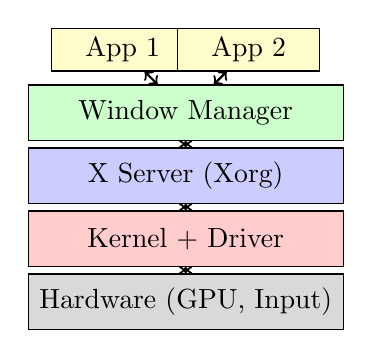
\begin{tikzpicture}[scale=0.8]
    % Hardware
    \node[draw, rectangle, fill=gray!30, minimum width=4cm, minimum height=0.7cm] (hw) at (0,0) {Hardware (GPU, Input)};
    
    % Kernel
    \node[draw, rectangle, fill=red!20, minimum width=4cm, minimum height=0.7cm] (kernel) at (0,1) {Kernel + Driver};
    
    % X Server
    \node[draw, rectangle, fill=blue!20, minimum width=4cm, minimum height=0.7cm] (xserver) at (0,2) {X Server (Xorg)};
    
    % Window Manager
    \node[draw, rectangle, fill=green!20, minimum width=4cm, minimum height=0.7cm] (wm) at (0,3) {Window Manager};
    
    % Applications
    \node[draw, rectangle, fill=yellow!20, minimum width=1.8cm, minimum height=0.5cm] (app1) at (-1,4) {App 1};
    \node[draw, rectangle, fill=yellow!20, minimum width=1.8cm, minimum height=0.5cm] (app2) at (1,4) {App 2};
    
    \draw[<->, thick] (hw) -- (kernel);
    \draw[<->, thick] (kernel) -- (xserver);
    \draw[<->, thick] (xserver) -- (wm);
    \draw[<->, thick] (wm) -- (app1);
    \draw[<->, thick] (wm) -- (app2);
\end{tikzpicture}

\vspace{0.3cm}

\textbf{File configurazione:}
\begin{itemize}
    \item \texttt{/etc/X11/xorg.conf} (legacy)
    \item \texttt{/etc/X11/xorg.conf.d/}
    \item Auto-configurazione moderna
\end{itemize}
\end{columns}
\end{frame}

% Slide 31: Wayland
\begin{frame}{Wayland: Il Futuro del Display}
\begin{columns}
\column{0.5\textwidth}
\textbf{Cos'è Wayland?}

\begin{itemize}
    \item Protocollo display moderno
    \item Sostituisce X11
    \item Più semplice, sicuro, performante
    \item Compositor-based
    \item Default in Fedora, Ubuntu (opzionale)
\end{itemize}

\vspace{0.3cm}

\textbf{Vantaggi vs X11:}

\begin{itemize}
    \item Meno latency
    \item Migliore sicurezza
    \item Rendering più efficiente
    \item Supporto touchscreen migliore
    \item Codice più pulito
    \item HiDPI nativo
\end{itemize}

\column{0.5\textwidth}
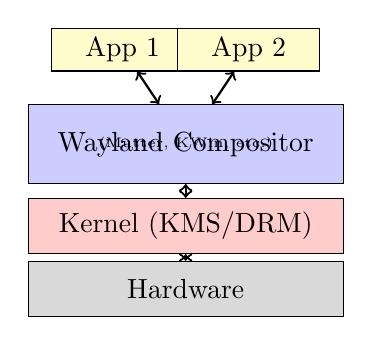
\begin{tikzpicture}[scale=0.8]
    % Hardware
    \node[draw, rectangle, fill=gray!30, minimum width=4cm, minimum height=0.7cm] (hw) at (0,0) {Hardware};
    
    % Kernel
    \node[draw, rectangle, fill=red!20, minimum width=4cm, minimum height=0.7cm] (kernel) at (0,1) {Kernel (KMS/DRM)};
    
    % Wayland Compositor
    \node[draw, rectangle, fill=blue!20, minimum width=4cm, minimum height=1cm] (comp) at (0,2.3) {Wayland Compositor};
    \node[font=\tiny] at (0,2.3) {(Mutter, KWin, etc.)};
    
    % Applications
    \node[draw, rectangle, fill=yellow!20, minimum width=1.8cm, minimum height=0.5cm] (app1) at (-1,3.8) {App 1};
    \node[draw, rectangle, fill=yellow!20, minimum width=1.8cm, minimum height=0.5cm] (app2) at (1,3.8) {App 2};
    
    \draw[<->, thick] (hw) -- (kernel);
    \draw[<->, thick] (kernel) -- (comp);
    \draw[<->, thick] (comp) -- (app1);
    \draw[<->, thick] (comp) -- (app2);
\end{tikzpicture}

\vspace{0.3cm}

\textbf{Compositor popolari:}
\begin{itemize}
    \item Mutter (GNOME)
    \item KWin (KDE Plasma)
    \item Sway (i3-like)
    \item Weston (riferimento)
\end{itemize}
\end{columns}
\end{frame}

% Slide 32: X11 vs Wayland
\begin{frame}{Confronto X11 vs Wayland}
\begin{table}
\small
\begin{tabular}{p{3cm}p{5cm}p{5cm}}
\toprule
\textbf{Aspetto} & \textbf{X11} & \textbf{Wayland} \\
\midrule
Architettura & Client-Server separati & Compositor unificato \\
\midrule
Performance & Buone, ma overhead & Migliori, meno latency \\
\midrule
Sicurezza & App vedono tutto schermo & Isolamento tra app \\
\midrule
Network & Supporto nativo & Tramite soluzioni esterne \\
\midrule
Compatibilità & Eccellente, legacy & Buona, in miglioramento \\
\midrule
Complessità & Codice vecchio, complesso & Codice moderno, pulito \\
\midrule
Screen recording & Facile & Richiede portali \\
\midrule
HiDPI & Supporto aggiunto dopo & Nativo \\
\bottomrule
\end{tabular}
\end{table}

\vspace{0.3cm}

\textbf{Quando usare X11:}
\begin{itemize}
    \item Software legacy incompatibile
    \item Necessità screen sharing/recording specifici
    \item Driver proprietari vecchi (NVIDIA)
    \item Applicazioni remote X11
\end{itemize}

\textbf{Quando usare Wayland:}
\begin{itemize}
    \item Hardware moderno
    \item Sicurezza prioritaria
    \item Migliori performance
    \item Touchscreen/gestures
\end{itemize}
\end{frame}

% Slide 33: Desktop Environment - GNOME
\begin{frame}{GNOME: Desktop Environment Moderno}
\begin{columns}
\column{0.5\textwidth}
\textbf{Caratteristiche:}

\begin{itemize}
    \item Default: Ubuntu, Fedora, Debian
    \item Interfaccia minimalista
    \item Workflow basato su Activities
    \item GNOME Shell (interfaccia)
    \item Mutter (compositor)
    \item GTK toolkit
\end{itemize}

\vspace{0.3cm}

\textbf{Componenti principali:}

\begin{itemize}
    \item Top Bar
    \item Activities Overview
    \item Dash (launcher applicazioni)
    \item Workspaces (spazi di lavoro)
    \item Notifiche
    \item System Menu
\end{itemize}

\column{0.5\textwidth}
\textbf{Applicazioni core:}

\begin{itemize}
    \item Files (Nautilus)
    \item Terminal (GNOME Terminal)
    \item Text Editor (gedit/GNOME Text Editor)
    \item Calendar
    \item Contacts
    \item Photos
    \item Music
    \item Videos (Totem)
\end{itemize}

\vspace{0.3cm}

\textbf{Personalizzazione:}

\begin{itemize}
    \item GNOME Tweaks
    \item Extensions
    \item Themes GTK/Shell
    \item Icone
    \item Fonts
\end{itemize}

\vspace{0.2cm}

\textbf{Requisiti:}
\begin{itemize}
    \item RAM: 4+ GB
    \item Grafica accelerata raccomandata
\end{itemize}
\end{columns}
\end{frame}

% Slide 34: Desktop Environment - KDE Plasma
\begin{frame}{KDE Plasma: Potente e Personalizzabile}
\begin{columns}
\column{0.5\textwidth}
\textbf{Caratteristiche:}

\begin{itemize}
    \item Altamente personalizzabile
    \item Look moderno (simile Windows)
    \item Qt toolkit
    \item KWin compositor
    \item Tante funzionalità integrate
    \item Leggero (contrariamente al mito)
\end{itemize}

\vspace{0.3cm}

\textbf{Componenti:}

\begin{itemize}
    \item Plasma Desktop/Panel
    \item Widgets/Plasmoids
    \item KRunner (launcher)
    \item System Settings
    \item Activities
    \item Virtual Desktops
\end{itemize}

\column{0.5\textwidth}
\textbf{Applicazioni KDE:}

\begin{itemize}
    \item Dolphin (file manager)
    \item Konsole (terminal)
    \item Kate (editor testo)
    \item Okular (documenti PDF)
    \item Gwenview (immagini)
    \item Spectacle (screenshot)
    \item Discover (software center)
    \item KMail, Kontact, Krita, Kdenlive
\end{itemize}

\vspace{0.3cm}

\textbf{Personalizzazione:}

\begin{itemize}
    \item System Settings completo
    \item Themes globali
    \item Window decorations
    \item Effetti desktop
    \item Widget ovunque
    \item Script e automazioni
\end{itemize}
\end{columns}
\end{frame}

% Slide 35: Altri Desktop Environment
\begin{frame}{Altri Desktop Environment}
\begin{columns}
\column{0.5\textwidth}
\textbf{Xfce}
\begin{itemize}
    \item Leggero e veloce
    \item Tradizionale
    \item GTK-based
    \item Molto stabile
    \item RAM: 1-2 GB
    \item Default: Xubuntu
\end{itemize}

\vspace{0.3cm}

\textbf{MATE}
\begin{itemize}
    \item Fork di GNOME 2
    \item Interfaccia classica
    \item Medio-leggero
    \item Familiare per utenti Windows XP
    \item Default: Ubuntu MATE
\end{itemize}

\vspace{0.3cm}

\textbf{Cinnamon}
\begin{itemize}
    \item Creato da Linux Mint
    \item Elegante, moderno
    \item Simile a Windows 7/10
    \item GTK-based
    \item Buon compromesso
\end{itemize}

\column{0.5\textwidth}
\textbf{LXQt}
\begin{itemize}
    \item Leggerissimo
    \item Qt-based
    \item Merge di LXDE e Razor-qt
    \item Per hardware limitato
    \item RAM: 512 MB
    \item Default: Lubuntu
\end{itemize}

\vspace{0.3cm}

\textbf{Budgie}
\begin{itemize}
    \item Moderno ed elegante
    \item Sviluppato per Solus
    \item Simile a GNOME
    \item GNOME-based
\end{itemize}

\vspace{0.3cm}

\textbf{Deepin DE}
\begin{itemize}
    \item Bellissimo visivamente
    \item Stile macOS/Windows
    \item Cinese
    \item Risorse medie
\end{itemize}
\end{columns}

\vspace{0.3cm}
\textbf{Scelta DE:} Dipende da risorse hardware, gusti estetici, workflow preferito
\end{frame}

% Slide 36: Window Manager
\begin{frame}{Window Manager Standalone}
\begin{columns}
\column{0.5\textwidth}
\textbf{Cos'è un WM?}

\begin{itemize}
    \item Gestisce solo finestre
    \item Più leggero di DE completo
    \item Maggiore controllo
    \item Configurazione manuale
    \item Per utenti avanzati
\end{itemize}

\vspace{0.3cm}

\textbf{Tipi di WM:}

\begin{enumerate}
    \item \textbf{Stacking} (floating)
    \begin{itemize}
        \item Finestre sovrapposte
        \item Es: Openbox, Fluxbox
    \end{itemize}
    
    \item \textbf{Tiling}
    \begin{itemize}
        \item Finestre affiancate
        \item Nessuna sovrapposizione
        \item Es: i3, bspwm, awesome
    \end{itemize}
    
    \item \textbf{Dynamic}
    \begin{itemize}
        \item Combinazione dei due
        \item Es: dwm, xmonad
    \end{itemize}
\end{enumerate}

\column{0.5\textwidth}
\textbf{WM popolari:}

\textbf{i3wm:}
\begin{itemize}
    \item Tiling, molto popolare
    \item Configurazione semplice
    \item Keyboard-driven
    \item Documentazione eccellente
\end{itemize}

\textbf{Openbox:}
\begin{itemize}
    \item Stacking, leggerissimo
    \item Altamente configurabile
    \item Menu contestuali
\end{itemize}

\textbf{bspwm:}
\begin{itemize}
    \item Tiling minimalista
    \item Configurazione via scripting
    \item Molto flessibile
\end{itemize}

\vspace{0.3cm}

\textbf{Componenti aggiuntivi necessari:}
\begin{itemize}
    \item Panel/Bar (polybar, i3bar)
    \item Launcher (rofi, dmenu)
    \item Compositor (picom)
    \item Wallpaper setter
\end{itemize}
\end{columns}
\end{frame}

% Slide 37: Display Manager
\begin{frame}[fragile]{Display Manager (Login Manager)}
\begin{columns}
\column{0.5\textwidth}
\textbf{Cos'è un Display Manager?}

\begin{itemize}
    \item Schermata di login grafica
    \item Avvia sessione X11/Wayland
    \item Gestisce utenti
    \item Scelta Desktop Environment
\end{itemize}

\vspace{0.3cm}

\textbf{Display Manager comuni:}

\textbf{GDM (GNOME)}
\begin{itemize}
    \item Default GNOME
    \item Wayland-ready
    \item Integrato con GNOME
\end{itemize}

\textbf{LightDM}
\begin{itemize}
    \item Leggero, veloce
    \item Molto configurabile
    \item Greeters personalizzabili
\end{itemize}

\textbf{SDDM (KDE)}
\begin{itemize}
    \item Default KDE Plasma
    \item Qt-based
    \item Temi personalizzabili
\end{itemize}

\column{0.5\textwidth}
\textbf{Cambiare Display Manager:}

\begin{lstlisting}[language=bash, basicstyle=\ttfamily\tiny, escapeinside={(*}{*)}]
(*\#*) Debian/Ubuntu
sudo dpkg-reconfigure gdm3
(*\#*) o
sudo dpkg-reconfigure lightdm

(*\#*) Fedora
sudo systemctl disable gdm
sudo systemctl enable sddm
sudo systemctl set-default graphical.target
\end{lstlisting}

\vspace{0.3cm}

\textbf{Avvio senza DM:}

\begin{lstlisting}[language=bash, basicstyle=\ttfamily\tiny, escapeinside={(*}{*)}]
(*\#*) Disabilitare DM
sudo systemctl disable gdm

(*\#*) Avviare X manualmente
startx

(*\#*) Con .xinitrc
echo "exec i3" > ~/.xinitrc
\end{lstlisting}

\vspace{0.2cm}

\textbf{File di configurazione:}
\begin{itemize}
    \item GDM: \texttt{/etc/gdm3/}
    \item LightDM: \texttt{/etc/lightdm/}
    \item SDDM: \texttt{/etc/sddm.conf}
\end{itemize}
\end{columns}
\end{frame}

% Slide 38: Driver Grafici
\begin{frame}[fragile]{Driver Grafici in Linux}
\begin{columns}
\column{0.5\textwidth}
\textbf{Driver Open Source:}

\textbf{Intel:}
\begin{itemize}
    \item Driver: i915 (kernel)
    \item Mesa (userspace)
    \item Inclusi di default
    \item Ottime performance
\end{itemize}

\textbf{AMD:}
\begin{itemize}
    \item Driver: amdgpu (kernel)
    \item Mesa + RADV/RadeonSI
    \item Molto buoni
    \item Performance eccellenti
\end{itemize}

\textbf{NVIDIA:}
\begin{itemize}
    \item Nouveau (limitato)
    \item Performance base
    \item Niente power management ottimale
\end{itemize}

\column{0.5\textwidth}
\textbf{Driver Proprietari NVIDIA:}

\begin{lstlisting}[language=bash, basicstyle=\ttfamily\tiny, escapeinside={(*}{*)}]
(*\#*) Ubuntu
sudo ubuntu-drivers devices
sudo ubuntu-drivers autoinstall
(*\#*) o manuale
sudo apt install nvidia-driver-535

(*\#*) Fedora
sudo dnf install akmod-nvidia
sudo dnf install xorg-x11-drv-nvidia-cuda

(*\#*) Verificare installazione
nvidia-smi
\end{lstlisting}

\vspace{0.3cm}

\textbf{Problemi NVIDIA + Wayland:}
\begin{itemize}
    \item Supporto in miglioramento
    \item GBM necessario (driver 495+)
    \item Alcune distro disabilitano Wayland
\end{itemize}

\vspace{0.2cm}

\textbf{Hybrid Graphics:}
\begin{itemize}
    \item Laptop con Intel + NVIDIA
    \item Prime/Optimus
    \item Bumblebee (vecchio)
\end{itemize}
\end{columns}
\end{frame}

% Slide 39: Risoluzione Problemi
\begin{frame}[fragile]{Risoluzione Problemi Comuni}
\begin{columns}
\column{0.5\textwidth}
\textbf{Problemi di boot:}

\begin{itemize}
    \item \textbf{GRUB non appare}
    \begin{itemize}
        \item Reinstallare GRUB
        \item Verificare UEFI/Legacy
    \end{itemize}
    
    \item \textbf{Kernel panic}
    \begin{itemize}
        \item Boot con kernel precedente
        \item Verificare driver
    \end{itemize}
\end{itemize}

\vspace{0.2cm}

\textbf{Problemi grafici:}

\begin{lstlisting}[language=bash, basicstyle=\ttfamily\tiny, escapeinside={(*}{*)}]
(*\#*) Avviare in modalità testo
(*\#*) Al boot: Esc/Shift → 'e' su GRUB
(*\#*) Aggiungere: systemd.unit=multi-user.target

(*\#*) Reinstallare driver
sudo apt install --reinstall xserver-xorg

(*\#*) Log X11
cat /var/log/Xorg.0.log
\end{lstlisting}

\column{0.5\textwidth}
\textbf{Problemi di rete:}

\begin{lstlisting}[language=bash, basicstyle=\ttfamily\tiny, escapeinside={(*}{*)}]
(*\#*) Verificare stato
ip addr
nmcli device status

(*\#*) Riavviare NetworkManager
sudo systemctl restart NetworkManager

(*\#*) WiFi non funziona
sudo apt install linux-firmware
\end{lstlisting}

\vspace{0.2cm}

\textbf{Sistema lento:}

\begin{lstlisting}[language=bash, basicstyle=\ttfamily\tiny, escapeinside={(*}{*)}]
(*\#*) Verificare uso risorse
htop
iotop

(*\#*) Disabilitare servizi inutili
systemctl list-unit-files --state=enabled
sudo systemctl disable servizio

(*\#*) Pulire sistema
sudo apt autoremove
sudo apt autoclean
journalctl --vacuum-size=100M
\end{lstlisting}
\end{columns}
\end{frame}

% Slide 40: Best Practices
\begin{frame}{Best Practices: Manutenzione Sistema}
\begin{columns}
\column{0.5\textwidth}
\textbf{Backup regolari:}

\begin{itemize}
    \item Dati utente (/home)
    \item Configurazioni (/etc)
    \item Lista pacchetti installati
    \item Tool: rsync, Timeshift, Déjà Dup
\end{itemize}

\vspace{0.3cm}

\textbf{Aggiornamenti:}

\begin{itemize}
    \item Aggiornare regolarmente
    \item Sicurezza = priorità
    \item Leggere changelog importanti
    \item Testare dopo major updates
\end{itemize}

\vspace{0.3cm}

\textbf{Sicurezza:}

\begin{itemize}
    \item Password forti
    \item Firewall attivo (ufw)
    \item Non usare root per uso normale
    \item SSH con chiavi, non password
    \item Cifrare dati sensibili
\end{itemize}

\column{0.5\textwidth}
\textbf{Ottimizzazione:}

\begin{itemize}
    \item Rimuovere software inutilizzato
    \item Pulire cache periodicamente
    \item Monitorare spazio disco
    \item Disabilitare servizi non necessari
    \item SSD: abilitare TRIM
\end{itemize}

\vspace{0.3cm}

\textbf{Documentazione:}

\begin{itemize}
    \item Annotare modifiche sistema
    \item Salvare comandi utili
    \item Documentare problemi risolti
    \item Tenere log configurazioni custom
\end{itemize}

\vspace{0.3cm}

\textbf{Repository:}

\begin{itemize}
    \item Usare repo ufficiali quando possibile
    \item Attenzione a PPA/COPR non mantenuti
    \item Verificare firma pacchetti
    \item Non mischiare repo distro diverse
\end{itemize}
\end{columns}
\end{frame}

% Slide 41: Strumenti Utili
\begin{frame}[fragile]{Strumenti Utili per Amministrazione}
\begin{columns}
\column{0.5\textwidth}
\textbf{Monitoraggio sistema:}

\begin{lstlisting}[language=bash, basicstyle=\ttfamily\tiny, escapeinside={(*}{*)}]
(*\#*) Processi
htop
top

(*\#*) Disco
df -h
du -sh *
ncdu

(*\#*) Memoria
free -h

(*\#*) Rete
iftop
nethogs
\end{lstlisting}

\vspace{0.3cm}

\textbf{Log:}

\begin{lstlisting}[language=bash, basicstyle=\ttfamily\tiny, escapeinside={(*}{*)}]
(*\#*) Journalctl
journalctl -xe
journalctl -f
journalctl -u servizio

(*\#*) Log tradizionali
/var/log/syslog
/var/log/auth.log
\end{lstlisting}

\column{0.5\textwidth}
\textbf{Backup:}

\begin{lstlisting}[language=bash, basicstyle=\ttfamily\tiny, escapeinside={(*}{*)}]
(*\#*) Timeshift (snapshot sistema)
sudo apt install timeshift

(*\#*) Rsync backup
rsync -av /source/ /destination/

(*\#*) Compressione
tar -czf backup.tar.gz /directory/
\end{lstlisting}

\vspace{0.3cm}

\textbf{Utilities:}

\begin{itemize}
    \item \textbf{bleachbit} - Pulizia sistema
    \item \textbf{gparted} - Partizionamento GUI
    \item \textbf{synaptic} - Package manager GUI
    \item \textbf{stacer} - Ottimizzazione sistema
    \item \textbf{neofetch} - Info sistema
\end{itemize}
\end{columns}
\end{frame}

% Slide 42: Risorse Online
\begin{frame}{Risorse per Approfondire}
\begin{columns}
\column{0.5\textwidth}
\textbf{Documentazione Ufficiale:}

\begin{itemize}
    \item Ubuntu: \texttt{help.ubuntu.com}
    \item Debian: \texttt{debian.org/doc}
    \item Fedora: \texttt{docs.fedoraproject.org}
    \item ArchWiki (universale): \texttt{wiki.archlinux.org}
\end{itemize}

\vspace{0.3cm}

\textbf{Community:}

\begin{itemize}
    \item Ask Ubuntu
    \item Reddit: r/linux, r/Ubuntu, r/Fedora
    \item Forum ufficiali distribuzioni
    \item IRC/Discord channels
    \item Stack Exchange Unix/Linux
\end{itemize}

\column{0.5\textwidth}
\textbf{Guide e Tutorial:}

\begin{itemize}
    \item Linux Journey
    \item The Linux Documentation Project
    \item DigitalOcean Tutorials
    \item Linux Academy / A Cloud Guru
\end{itemize}

\vspace{0.3cm}

\textbf{Canali YouTube:}

\begin{itemize}
    \item LearnLinuxTV
    \item Chris Titus Tech
    \item The Linux Experiment
    \item DistroTube
    \item Tecmint
\end{itemize}

\vspace{0.3cm}

\textbf{Podcast:}

\begin{itemize}
    \item Linux Unplugged
    \item Late Night Linux
    \item Destination Linux
\end{itemize}
\end{columns}
\end{frame}

% Slide 43: Conclusioni
\begin{frame}{Conclusioni}
\textbf{Punti chiave:}

\begin{enumerate}
    \item \textbf{Installazione:} Processo guidato per Ubuntu, più controllo con Debian, moderno con Fedora
    
    \item \textbf{Gestione pacchetti:} APT (Debian/Ubuntu), DNF (Fedora), più Flatpak/Snap per app universali
    
    \item \textbf{Aggiornamenti:} Regolari per sicurezza, upgrade versione ben pianificato
    
    \item \textbf{Sistemi grafici:} X11 maturo vs Wayland moderno, scelta DE per preferenze/risorse
    
    \item \textbf{Manutenzione:} Backup, aggiornamenti, sicurezza, documentazione
\end{enumerate}

\vspace{0.5cm}

\begin{center}
\Large{Linux offre flessibilità e controllo:\\scegliere la distribuzione e DE giusti\\per le proprie esigenze!}
\end{center}
\end{frame}

% Slide 44: Bibliografia
\begin{frame}{Bibliografia}
\small
\textbf{Libri:}
\begin{itemize}
    \item Shotts, W. (2019). \textit{The Linux Command Line} (2nd ed.). No Starch Press.
    \item Ward, B. (2021). \textit{How Linux Works} (3rd ed.). No Starch Press.
    \item Negus, C. (2020). \textit{Linux Bible} (10th ed.). Wiley.
    \item Blum, R., \& Bresnahan, C. (2020). \textit{Linux Command Line and Shell Scripting Bible} (4th ed.). Wiley.
\end{itemize}

\textbf{Documentazione Ufficiale:}
\begin{itemize}
    \item Ubuntu Documentation: \texttt{https://help.ubuntu.com/}
    \item Debian Administrator's Handbook: \texttt{https://debian-handbook.info/}
    \item Fedora Documentation: \texttt{https://docs.fedoraproject.org/}
    \item GNOME Documentation: \texttt{https://help.gnome.org/}
    \item KDE UserBase Wiki: \texttt{https://userbase.kde.org/}
\end{itemize}

\textbf{Riferimenti Tecnici:}
\begin{itemize}
    \item Debian Policy Manual: \texttt{https://www.debian.org/doc/debian-policy/}
    \item Fedora System Administrator's Guide
    \item Ubuntu Server Guide: \texttt{https://ubuntu.com/server/docs}
    \item Filesystem Hierarchy Standard: \texttt{https://refspecs.linuxfoundation.org/fhs.shtml}
    \item Wayland Documentation: \texttt{https://wayland.freedesktop.org/}
\end{itemize}
\end{frame}

% Slide 45: Riferimenti Aggiuntivi
\begin{frame}{Riferimenti Aggiuntivi}
\small
\textbf{Package Management:}
\begin{itemize}
    \item APT User's Guide: \texttt{https://www.debian.org/doc/manuals/apt-guide/}
    \item DNF Documentation: \texttt{https://dnf.readthedocs.io/}
    \item Flatpak Documentation: \texttt{https://docs.flatpak.org/}
    \item Snap Documentation: \texttt{https://snapcraft.io/docs}
\end{itemize}

\textbf{Desktop Environments:}
\begin{itemize}
    \item GNOME Human Interface Guidelines: \texttt{https://developer.gnome.org/hig/}
    \item KDE Plasma Documentation: \texttt{https://docs.kde.org/}
    \item Xfce Documentation: \texttt{https://docs.xfce.org/}
    \item MATE Desktop Wiki: \texttt{https://wiki.mate-desktop.org/}
\end{itemize}

\textbf{Display Servers:}
\begin{itemize}
    \item X.Org Documentation: \texttt{https://www.x.org/wiki/Documentation/}
    \item Wayland Book: \texttt{https://wayland-book.com/}
\end{itemize}

\textbf{Community Resources:}
\begin{itemize}
    \item ArchWiki (risorsa universale): \texttt{https://wiki.archlinux.org/}
    \item LinuxQuestions.org
    \item The Linux Documentation Project: \texttt{https://tldp.org/}
\end{itemize}
\end{frame}

\end{document}
